\documentclass[border=6pt]{standalone}
\usepackage{amsmath,amssymb}
\usepackage{tikz}
\usetikzlibrary{arrows.meta,calc,decorations.pathreplacing,patterns,shapes.geometric,positioning,shadings,plotmarks}

\begin{document}
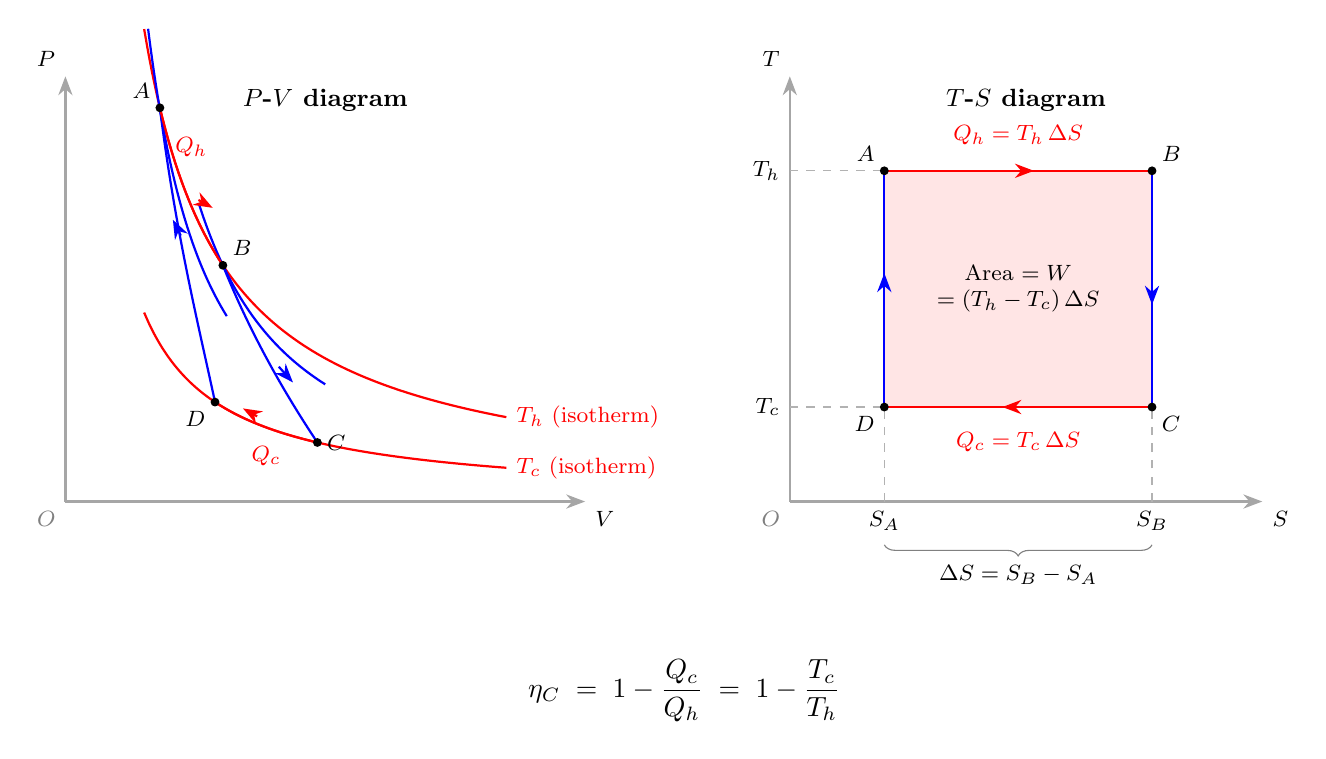
\begin{tikzpicture}[>={Stealth[length=2.4mm]}, font=\footnotesize]

%====================================================
%  LEFT PANEL : P - V diagram of Carnot cycle
%====================================================
\begin{scope}[local bounding box=PV]
  % Axes
  \draw[->, gray!70, thick] (0,0) -- (6.6,0) node[below right, black]{$V$};
  \draw[->, gray!70, thick] (0,0) -- (0,5.4) node[above left, black]{$P$};
  \node[gray, anchor=north east] at (0,0) {$O$};

  % --- Two isotherms (PV = const, red) ---
  % Hot isotherm  P = k_h / V , passing through high pressures
  % Cold isotherm P = k_c / V , passing through lower pressures
  % Choose constants so curves are clearly separated.
  % Hot: k_h = 6.0,  Cold: k_c = 2.4
  \draw[red, thick, domain=1.0:5.6, smooth, samples=80]
        plot (\x, {6.0/\x}) node[right, red]{$T_h$ (isotherm)};
  \draw[red, thick, domain=1.0:5.6, smooth, samples=80]
        plot (\x, {2.4/\x}) node[right, red]{$T_c$ (isotherm)};

  % --- Two adiabats (PV^gamma = const, blue, steeper) ---
  % gamma = 1.4
  % Adiabat 1 (B->C): passes through B = (2.0, 3.0) -> const = 3.0 * 2^1.4
  % Adiabat 2 (D->A): passes through A = (1.2, 5.0) -> const = 5.0 * 1.2^1.4
  % Compute constants numerically:
  %   2^1.4 ~ 2.6390  -> const1 = 7.917
  %   1.2^1.4 ~ 1.2856 -> const2 = 6.428
  \draw[blue, thick, domain=1.7:3.3, smooth, samples=80]
        plot (\x, {7.917/(\x^1.4)});
  \draw[blue, thick, domain=1.05:2.05, smooth, samples=80]
        plot (\x, {6.428/(\x^1.4)});

  % --- Vertices A,B,C,D ---
  % A on hot isotherm:  V=1.2, P=6.0/1.2 = 5.0
  % B on hot isotherm:  V=2.0, P=6.0/2.0 = 3.0
  % C on cold isotherm: V_C from adiabat1 -> 7.917/V^1.4 = 2.4/V => V^0.4 = 7.917/2.4 = 3.299
  %    V_C = 3.299^(1/0.4) = 3.299^2.5 ~ 19.6  ... too large; rescale.
  % We'll just place visually consistent points (figure is qualitative geometry).
  \coordinate (A) at (1.2, 5.0);
  \coordinate (B) at (2.0, 3.0);
  \coordinate (C) at (3.2, {2.4/3.2});   % on cold isotherm -> (3.2, 0.75)
  \coordinate (D) at (1.9, {2.4/1.9});   % on cold isotherm -> (1.9, 1.263)

  % Re-draw adiabats so they actually connect B->C and D->A visually
  % Use Bezier-like curves that match steeper-than-isotherm visual.
  \draw[blue, thick] (B) .. controls (2.4,2.0) and (2.9,1.2) .. (C);
  \draw[blue, thick] (D) .. controls (1.7,2.2) and (1.4,3.4) .. (A);

  % Draw isothermal arcs explicitly between vertices on top of curves
  \draw[red, thick, domain=1.2:2.0, smooth, samples=40]
        plot (\x, {6.0/\x});
  \draw[red, thick, domain=1.9:3.2, smooth, samples=40]
        plot (\x, {2.4/\x});

  % Vertex dots and labels
  \foreach \pt/\lab/\pos in {A/A/above left, B/B/above right, C/C/right, D/D/below left}{
    \fill[black] (\pt) circle (1.6pt);
    \node[\pos] at (\pt) {$\lab$};
  }

  % --- Direction arrows on segments ---
  \draw[->, red, thick] ($(A)!0.55!(B)$) ++(0.05,-0.07)
        -- ++(0.18,-0.10);
  \draw[->, blue, thick] ($(B)!0.55!(C)$) ++(0.05,-0.05)
        -- ++(0.18,-0.20);
  \draw[->, red, thick] ($(C)!0.55!(D)$) ++(-0.05,0.05)
        -- ++(-0.18,0.10);
  \draw[->, blue, thick] ($(D)!0.55!(A)$) ++(-0.05,0.06)
        -- ++(-0.10,0.20);

  % --- Q labels on isotherms ---
  \node[red, above] at ($(A)!0.5!(B) + (0.0,0.25)$) {$Q_h$};
  \node[red, below] at ($(C)!0.5!(D) + (0.0,-0.18)$) {$Q_c$};

  % Title
  \node[font=\small\bfseries] at (3.3,5.1) {$P\text{-}V$ diagram};
\end{scope}

%====================================================
%  RIGHT PANEL : T - S diagram (rectangle)
%====================================================
\begin{scope}[xshift=9.2cm, local bounding box=TS]
  % Axes
  \draw[->, gray!70, thick] (0,0) -- (6.0,0) node[below right, black]{$S$};
  \draw[->, gray!70, thick] (0,0) -- (0,5.4) node[above left, black]{$T$};
  \node[gray, anchor=north east] at (0,0) {$O$};

  % Coordinates of rectangle
  % Use S_A = 1.2, S_B = 4.6, T_c = 1.2, T_h = 4.2
  \coordinate (TA) at (1.2, 4.2);
  \coordinate (TB) at (4.6, 4.2);
  \coordinate (TC) at (4.6, 1.2);
  \coordinate (TD) at (1.2, 1.2);

  % Shaded area = net work
  \fill[red!10] (TA) rectangle (TC);

  % Top isotherm (red), bottom isotherm (red)
  \draw[red, thick] (TA) -- (TB);
  \draw[red, thick] (TD) -- (TC);
  % Vertical adiabats (blue)
  \draw[blue, thick] (TB) -- (TC);
  \draw[blue, thick] (TD) -- (TA);

  % Tick marks and dashed guides
  \draw[gray!60, dashed] (0,4.2) -- (TA) node[pos=0, left, black]{$T_h$};
  \draw[gray!60, dashed] (0,1.2) -- (TD) node[pos=0, left, black]{$T_c$};
  \draw[gray!60, dashed] (1.2,0) -- (TD) node[pos=0, below, black]{$S_A$};
  \draw[gray!60, dashed] (4.6,0) -- (TC) node[pos=0, below, black]{$S_B$};

  % Vertices
  \foreach \pt/\lab/\pos in {TA/A/above left, TB/B/above right, TC/C/below right, TD/D/below left}{
    \fill[black] (\pt) circle (1.6pt);
    \node[\pos] at (\pt) {$\lab$};
  }

  % Direction arrows (clockwise: A->B top, B->C right, C->D bottom, D->A left)
  \draw[->, red, thick]  ($(TA)!0.50!(TB)$) ++(-0.10,0) -- ++(0.30,0);
  \draw[->, blue, thick] ($(TB)!0.50!(TC)$) ++(0,0.10) -- ++(0,-0.30);
  \draw[->, red, thick]  ($(TC)!0.50!(TD)$) ++(0.10,0) -- ++(-0.30,0);
  \draw[->, blue, thick] ($(TD)!0.50!(TA)$) ++(0,-0.10) -- ++(0,0.30);

  % Labels for heats and work
  \node[red, above] at ($(TA)!0.5!(TB) + (0,0.20)$) {$Q_h = T_h\,\Delta S$};
  \node[red, below] at ($(TC)!0.5!(TD) + (0,-0.20)$) {$Q_c = T_c\,\Delta S$};
  \node[align=center] at ($(TA)!0.5!(TC)$) {Area $= W$\\$=(T_h-T_c)\,\Delta S$};

  % Width brace under rectangle for Delta S
  \draw[decorate, decoration={brace, amplitude=4pt, mirror}, gray]
        (1.2,-0.55) -- (4.6,-0.55) node[midway, below=4pt, black]{$\Delta S = S_B - S_A$};

  % Title
  \node[font=\small\bfseries] at (3.0,5.1) {$T\text{-}S$ diagram};
\end{scope}

%====================================================
%  Common caption / formula under both panels
%====================================================
\node[font=\normalsize] at ($(PV.south)!0.5!(TS.south) + (0,-1.6)$)
  {$\displaystyle \eta_C \;=\; 1 - \frac{Q_c}{Q_h} \;=\; 1 - \frac{T_c}{T_h}$};

\end{tikzpicture}
\end{document}
